\documentclass{report}
\usepackage[utf8]{inputenc}
\usepackage[T1]{fontenc}
\usepackage[pdftex]{graphicx}
\begin{document}
\section{Beregning av hodeposisjon}
Det finnes mange måter å beregne posisjon til et objekt i forhold til et annet.
Valg av fremgangsmåte tas på bakgrunn av egenskaper som blant annet kostnad, presisjon, bevegelsesområde og oppdateringshastighet.

For dette systemet er det ingen bestemte krav for presisjon(oppløsning) eller oppdateringshastighet. Likevel bør ikke systemet
føles hakkete, det vil si at både presisjonen og oppdateringshastigheten bør være høy nok til å unngå at bevegelse resulterer i
hakkete bevegelse eller etterslep i en eventuell 3d-scene.

Da kostnad er en av prioriteringene til dette systemet er bruk av Nintendo Wiimote, en relativt billig kontroller med
innebygd optisk sensor og tracking av infrarøde lys, vurdert. Nintendo Wiimote har en oppløsning på 786 432 piksler og en oppdateringshastighet 
på ? bilder i sekundet\ref{Wiimote hacking}. Tidlige tester antyder at oppløsningen til Wiimote er i nedre sjikt av hva som er
akseptabelt, i tillegg er bevegelsesområdet noe begrenset på grunn av en noe lav utsynsvinkel på 45 grader.

På grunn av dette vil det også ses på støtte for bruk av kamera med vilkårlig oppdateringshastighet og presisjon.
Spesifikt et Panasonic HD-kamera med ~2,1 megapiksler, 60 grader utsynsvinkel og 60 bilder i sekundet. En vidvinkellinse
kan også monteres for å bedre utsynsvinkelen.

Beregning av hodeposisjon vil, på grunn av valgene over, bestå av å bruke informasjon om pikselposisjon av infrarøde punkter
i et todimensjonalt bilde. For å forenkle denne beregningen brukes vinkelmål istedet for piksler, og det antas derfor
at det er mulig å omregne pikselmål til vinkler. Ved bruk av Wiimote er det antatt at det er et konstant antall radianer
mellom hver piksel: $$rpp = \frac{\frac{\pi}{4}}{1024}$$.

Det bør nevnes at motivasjonen ligger i å beregne hodeposisjonen, det vil si at interessen ligger i bevegelse langs tre akser,
men ikke rotasjon om aksene. Det er ikke dermed slik at det ikke er mulig å beregne hoderotasjonen, eller at brukeren ikke har
mulighet til å rotere hodet. Årsaken til at det er interessant å kun beregne hodeposisjon er på grunn av at det kun er disse
parametrene som er nødvendig for å få riktig perspektivprojeksjon i en 3d-scene, dette blir forklart mer dyptgående i \ref{3d}.

\section{En optisk sensor og to infrarøde punkter}
Når en optisk sensor og to infrarøde punkter er brukt, enten en wiimote eller et kamera, er det antatt følgende.
\begin{enumerate}
\item To infrarøde punkter er alltid observerbare fra optisk sensor. 
\item Disse punktene er montert på hver sin side av brukerens hode.
\item Det er en kjent avstand $l$ mellom punktene. 
\item Brukerens hode er alltid vendt vinkelrett på den rette linjen fra sensor til brukeren.
\item Sensoren er plassert horisontalt i midten av skjermen, enten rett over eller rett under skjermen.
\end{enumerate}
Punkt fire medfører at brukeren ikke har mulighet til å rotere hodet om y-aksen relativt til den rette linjen mot skjermplanet, og
brukeren har derfor fem frihetsgrader for bevegelse: side til side, opp og ned, inn mot og fra skjermen, rotasjon om z-aksen og rotasjon om x-aksen.

Da gjelder de følgende matematiske forholdene. Se figur.
	\begin{figure}[h]
	\centering
	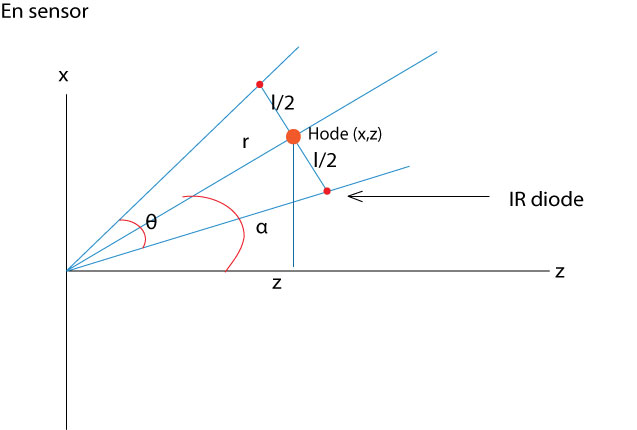
\includegraphics[width=0.80\textwidth]{graphics/Figur_en_sensor.jpg}
	\caption{Modell med en sensor}
	\label{fig:En_sensor}
	\end{figure}

\begin{eqnarray}\label{definition}
&r = \frac{l/2}{\tan( \theta/2 )}\\
&z = r \cos( \alpha )\\
&x = r \sin( \alpha )\\
&y = a + r \sin( \beta )
\end{eqnarray}
Parameteren $a$ angir forflytning langs y-aksen er tatt med for å kunne sette wiimote over eller under skjermen.
Det er ikke tatt med en forflytningsparameter for x-aksen, da det er antatt at sensor er posisjonert horisontalt i midten av skjermen.
Merk at $\beta$ er avhengig av vinkelen sensoren står i, ved at den for eksempel peker litt nedover.
Da er $\beta = \beta^\prime + b$, hvor $\beta^\prime$ er vinkel fra kameraets midtpunkt og $b$ må kalibreres når brukeren står i en kjent posisjon.

Antagelsen om at brukerens hode alltid er vendt mot sensoren er en følge av at kun to infrarøde punkter
utgjør beregningsgrunnlaget. Med tre infrarøde punkter kan man oppnå full bevegelsesfrihet, ved bruk
av algoritmer som \ref{hmm} eller \ref{hmm2}. Disse løsningene er iterative, og gir ikke eksakt(men veldig nære) løsninger.
Metoden beskrevet her, med antagelsen om at brukeren er vendt mot sensor, gir en eksakt løsning på lukket form.

\section{To optiske sensorer}

Når to optiske sensorer benyttes, er det antatt følgende.
\begin{enumerate}
\item Ett punkt, det samme punktet, er observerbart fra begge sensorene. 
\item Punktet ligger så nært hodets rotasjonssentrum at differansen er neglisjerbar.
\item Begge sensorene er plassert i samme høyde og med lik avstand $l/2$ fra midten av skjermen.
\end{enumerate}

Da gjelder følgende( Se figur \ref{fig:Figur_to_sensorer}).
	\begin{figure}[h]
	\centering
	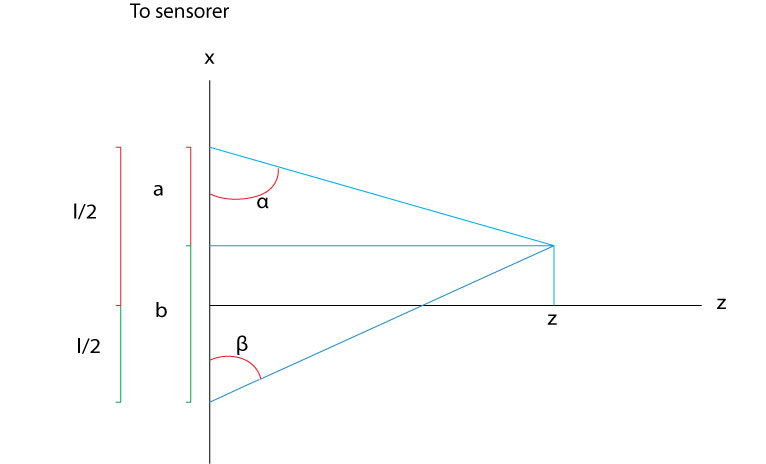
\includegraphics[width=0.80\textwidth]{graphics/Figur_2_sensorer.jpg}
	\caption{Illustrasjon to sensorer}
	\label{fig:Figur_to_sensorer}
	\end{figure}
\begin{eqnarray}\label{definition2}
&\frac{z}{a} = \tan( \alpha )\\
&\frac{z}{b} = \tan( \beta )\\
&l = a + b = z(\frac{1}{tan( \alpha )} + \frac{1}{tan( \beta )})
&z = \frac{l}{\frac{1}{\alpha} + \frac{1}{\beta}}\\
&x = \frac{l}{2} - \frac{z}{\tan( \alpha )}\\
&y = z\sin( \gamma )
\end{eqnarray}

Her er både $\alpha$, $\beta$ og $\gamma$ bestående av en sum av en offset og vinkelmål fra sensor, siden
sensorene står fritt til å peke inn mot eller ut fra skjermen, og helle litt nedover. Merk dog at 
det er antatt at begge sensorene har samme helling nedover, hvilket vil gjøre at $\gamma$ kan
brukes fra ett av sensorene eller midles fra begge.

\section{Tredimensjonal perspektivprojeksjon}
Et bruksområde som er muliggjort ved hjelp av hodetracking er å lage en fysisk riktig perspektivprojeksjon
i en virtuell tredimensjonal scene. En perspektivprojeksjon gjør at objekter langt unna tegnes
mindre enn nære objekter.
Dette gjøres gjennom to funksjoner i OpenGL. Disse funksjonene
manipulerer matrisene i OpenGL som transformerer koordinatene i 3d-scenen.
Den ene, gluLookAt, modifiserer modellmatrisen slik at det virtuelle kameraet eller øyet flyttes
og betraktningsretningen endres.  Den andre, glFrustum, modifiserer projeksjonsmatrisen slik at
man får en perspektivprojeksjon. Perspektivprojeksjonen bestemmes av dybden til nærplanet/klippeplanet
samt koordinatene til et rektangel på nærplanet.

I korte trekk flyttes "øyet" til hodeposisjonen, og betraktningsretningen settes til å være vinkelrett på
skjermplanet, det vil si at det virtuelle kamerat/øyet ikke roterer(et vindu vil ikke rotere om man ser på det fra en annen vinkel).
Så endres perspektivprojeksjonen, slik at hjørnekoordinatene på rektangelet på nærplanet sammenfaller med hjørnekoordinatene til
et virtuelt grid-rom. 

De følgende ligningene benyttes for å korrigere perspektivet(regne ut koordinatene til nærplanet) når øyet er flyttet til posisjonen x,y,z. Figur \ref{figur} viser denne sammenhengen.
	\begin{figure}[h]
	\centering
	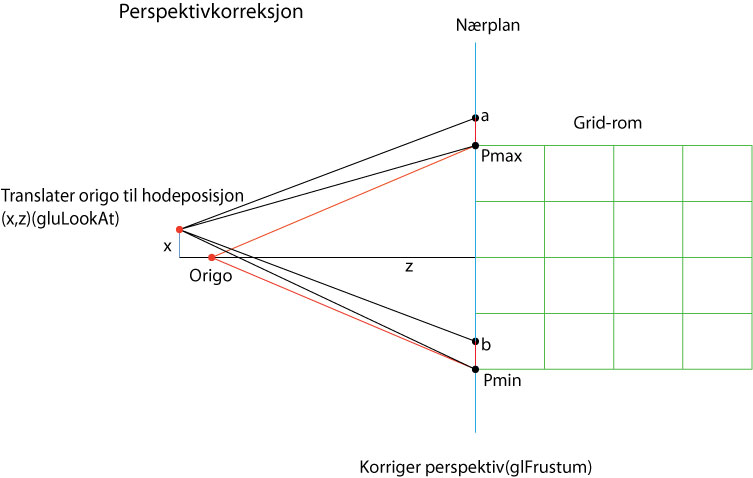
\includegraphics[width=0.80\textwidth]{graphics/Perspektivkorreksjon.jpg}
	\caption{HDMI-kontakt (venstre) og kabel (høyre)}
	\label{fig:hdmi}
	\end{figure}
\begin{eqnarray}
&p_{min} = b-x\\
&p_{max} = a-x
\end{eqnarray}
En vanlig verdi for a = 1/2, b=-1/2.
For y-aksen gjelder figur og ligninger med x utbyttet med y.

\section{Illusjonen}
En av målsetningene til prosjektgruppa var å produsere en eller flere demonstrasjonsprogrammer
som viser hvordan hodetracking kan brukes. Johnny Chung demonstrerer i en video på youtube
hvordan man kan få et objekt til å tilsynelatende bryte skjermflaten og sveve ut i rommet foran skjermen.
Denne illusjonen ble gjenskapt i produktet. Hvordan denne effekten oppstår kan kanskje en psykolog forklare
best, men rent teknisk oppnås denne effekten ved å angi dybden til nærplanet/klippeplanet, som nærmere enn
starten på grid-rommet og benytte en perspektivprojeksjonen som gjør at grid-rommet er kant-i-kant med skjermen.
Et objekt som befinner seg lenger frem enn skjermkantene vil da likevel tegnes på grunn av et nærmere nærplan.
I demonstrasjonen tegnes en linje fra bakveggen i rommet til objektet, sammenligner man denne linjen med linjene
i grid-rommet vil man se at linjen til objektet later til å være lenger, og dette forsterker inntrykket av at
objektet er lenger ut i rommet enn skjermflaten. 
Følgende ligninger brukes for å regne ut et nærmere nærplan. Se også figur \ref{figur}.
Definer $d$ som dybden til ønsket nærplan.
\begin{eqnarray}
&p_{min} = d\frac{b-x}{z}\\
&p_{max} = d\frac{a-x}{z}
\end{eqnarray}
For y-aksen gjelder figur og ligninger med x utbyttet med y.

	\begin{figure}[h]
	\centering
	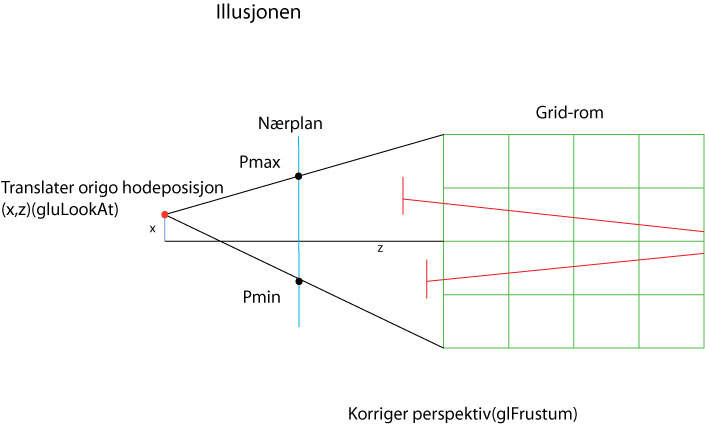
\includegraphics[width=0.80\textwidth]{graphics/Illusjonen.jpg}
	\caption{Illustrasjon illusjon}
	\label{fig:illusjon}
	\end{figure}

\section{Evaluering - Sammenligning med andre}
Før og i  løpet av prosjektet har prosjektgruppa merket seg og blitt inspirert av andre som har implementert lignende
løsninger. Av disse har vi sett på videomateriale fra tidligere VR-landsbyer, samt Johnny Chung Lee, Ph.D ved Carnegie Mellon University.
Prosjektetgruppas hovedmål har hele tiden vært at produktet skal være en god teknologisk løsning på headtracking.
Sammenlignet med disse er det prosjektgruppas mening at Virins er en like god eller bedre teknologisk løsning.
To egenskaper ved Virins er stor bevegelsesfrihet, samt to former(modi) for bestemmelse av hodeposisjon begge med eksakt løsning på lukket form.


Etter gjennomsyn av Johnny Chungs implementasjon kan det trekkes noen sammenligninger med Virins.
\begin{enumerate}
\item Virins tilbyr bruk av trianguleringsberegning når to sensorer benyttes(med full bevegelsesfrihet) samt en modell for beregning med en sensor hvor det er antatt at brukerens hode alltid er vendt mot sensoren.
\item Den matematiske modellen for beregning av hodeposisjon fra to lyspunkt er annerledes. (Bør dette utdypes? Basically, brukes R som Z. Som er rart!)
\item Det er tydelig at Johnny Chungs kode er ment primært som et eksempel på hvordan hodetracking og fysisk riktig perspektivprojeksjon
kan gjøres, og ikke et verktøy eller et rammeverk som kan brukes i andre prosjekter uten endring. Prosjektgruppa mener at Virins utgjør et rammeverk som godt kan brukes uten nevneverdig innsats som en modul for et software/spill-prosjekt som vil ta i bruk tracking av hode uten å implementere dette selv.
\end{enumerate}
Følgende er en sammenligning av Johnny Chungs implementasjon og implementasjon som er diskutert i denne rapporten.

\begin{tabular}{| l | p{4cm} | p{4cm} | }
\hline			
                        & \textbf{Virins}                                               & \textbf{Chung} \\
\hline
  Programmeringsspråk   & Java                                                          & C\# \\
\hline
  Plattformuavhengig    & Ja(OpenGL, Java)                                              & Nei(DirectX) \\
\hline
  Sensor                & Wiimote eller kamera                                          & Wiimote \\
\hline
  Modi                  & To wiimotes og triangulering eller en wiimote og kuleskall    & En wiimote og tilnærmet beregning \\
\hline  
\end{tabular}

Det bør nevnes at ved design av rammeverket ble det bestemt at JMF skulle brukes, siden dette er tilgjengelig på flere plattformer.
For å få tilgang til HDMI capture kortet ble vi nødt til å bruke et plattformspesifikt bibliotek for directshow, da HDMI capture kortet ikke var tilgjengelig ved bruk av JMF. Vanlige webkameraer ble testet og fungerte ved bruk av JMF, og rammeverket støtter
videokilder som er tilgjengelige gjennom JMF.  Rammeverket er derfor plattformuavhengig både ved bruk av Wiimotes og kamera, med mulighet til
å bruke et plattformspesifikt bibliotek for mer eksotiske videokilder som HDMI capture kort.

\end{document}
